\documentclass[a4paper, 12pt, english]{article}
\usepackage[utf8]{inputenc}
\usepackage{fancyhdr}
\usepackage{graphicx}
\usepackage{lastpage}
\usepackage{layout}
\usepackage{enumitem}
\usepackage{etoolbox}
\usepackage{amsmath}
\usepackage{mathptmx}
\usepackage[bottom]{footmisc}
\usepackage[includeheadfoot, left=3cm, right=3cm, top = 1.5 cm]{geometry}
\usepackage{minted}
\usemintedstyle{xcode}


\graphicspath{ {./answers/} }

\pagestyle{fancy}
\fancyhf{} 
\rhead{
    {\Large \textbf{Analysis and Design of Algorithms}}\\
    \textbf{CS2102} \\ 
    \textbf{Divide and Conquer Practice} \\ 
    \textbf{2020-II}
}
\lhead{
\includegraphics[width=4.6cm, keepaspectratio]{logo/utec}}
\rfoot{\textbf{\thepage}\hspace{1pt} of \textbf{\pageref{LastPage}}}
\cfoot{}

\setlength{\parindent}{0em}
\setlength{\headheight}{80pt}

\newcounter{problem}[section]
\newenvironment{problem}[3][]{\refstepcounter{problem}\par\medskip 

\textbf{Problem~\theproblem  ~~(#2) - 
\ifboolexpr{
  test {\ifdimless{1 pt}{#3 pt}}
}
{#3 points} % true
{#3 point} % false
} \newline\newline } {\medskip} 


\begin{document}

\textbf{Submission deadline}: December 10, 20:10\\ 

\begin{itemize}
    \item Write your answers (images) inside the \emph{answers} folder in order to generate a single PDF file. Replace the image files that are already included in the project. Do not change the file name.
    \item Read the questions carefully and write your answers clearly. Answers that are not legible and that doesn't follow the format will not have any score. 
\end{itemize}

\underline{Outcomes}:

\begin{enumerate}[label=\alph*.]
    \item Apply appropriate mathematical and related knowledge to computer science.
    \item Analyze problems and identify the appropriate computational requirements for its solution.
\end{enumerate}
\noindent\rule{\textwidth}{0.01pt}
\vspace{3mm}

\begin{problem}{Outcomes a, b}{4}
    Given the following expression:
    \begin{center}
        $T(n) = T(n/10) + T(9n/10) + \Theta(n)$
    \end{center}
    \begin{itemize}
        \item Sketch the recursion tree of $T(n)$ and indicate the exact height, the cost per level and the total cost of the tree.
        \item Based on the recursion tree above estimate a good upper and lower bound of $T(n)$. If no bounds can be found or are the same, express that clearly and explain the reason.
            %\item Prove by induction the upper and lower bounds obtained before
    \end{itemize}

    \begin{center}
        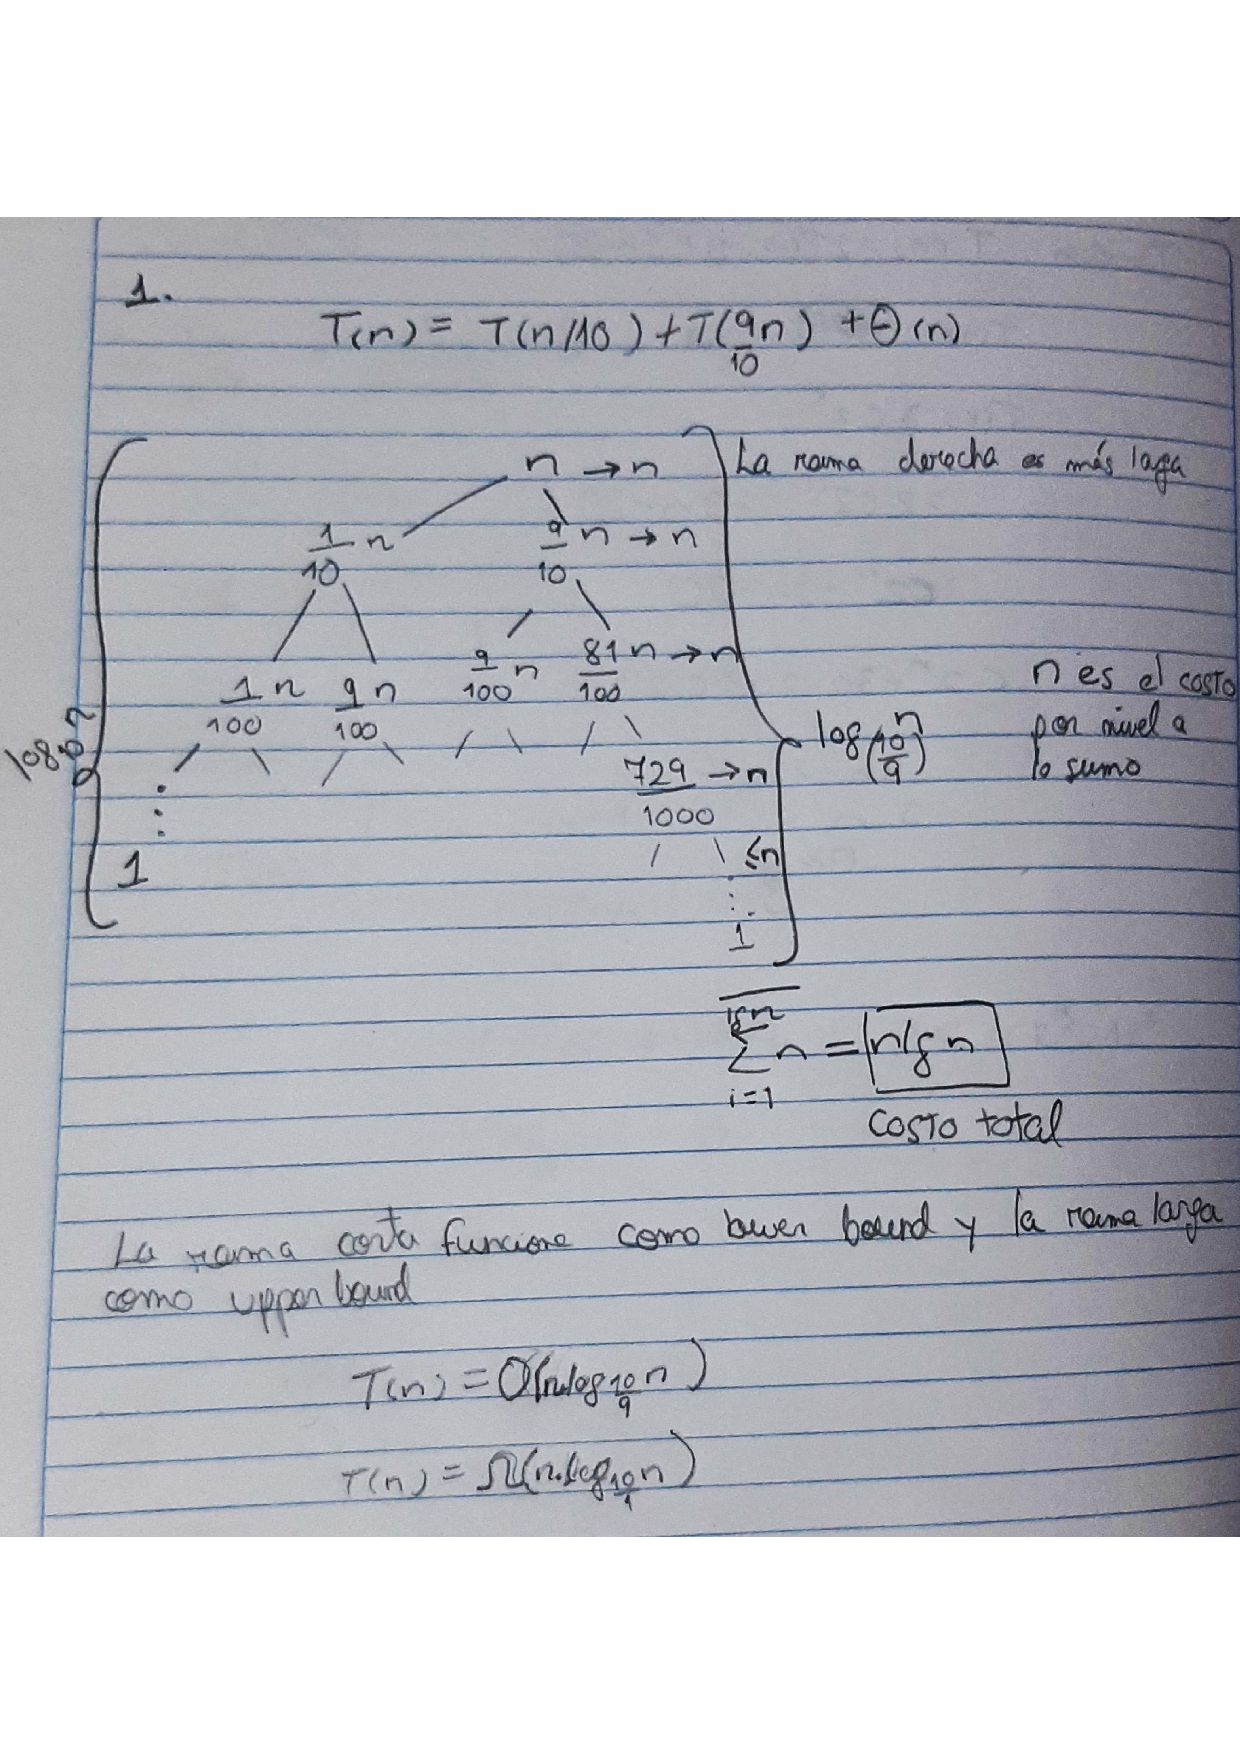
\includegraphics[width=0.9\linewidth]{problem1/problem1}%
    \end{center}
\end{problem}

\begin{problem}{Outcome b}{2}
    Consider that $T(n) = 0.5n^2 + 3n$ and for each of the items below indicate if the statement is true or false and justify the reason. 

    \begin{enumerate}
        \item $T(n) = O(n)$
        \item $T(n) = \Omega(n)$
        \item $2^{n+1} \leq O(2^n)$
        \item $T(n) = \Theta(n^2)$
            %\item $T(n) = \O(n^3)$
    \end{enumerate}

    \begin{center}
        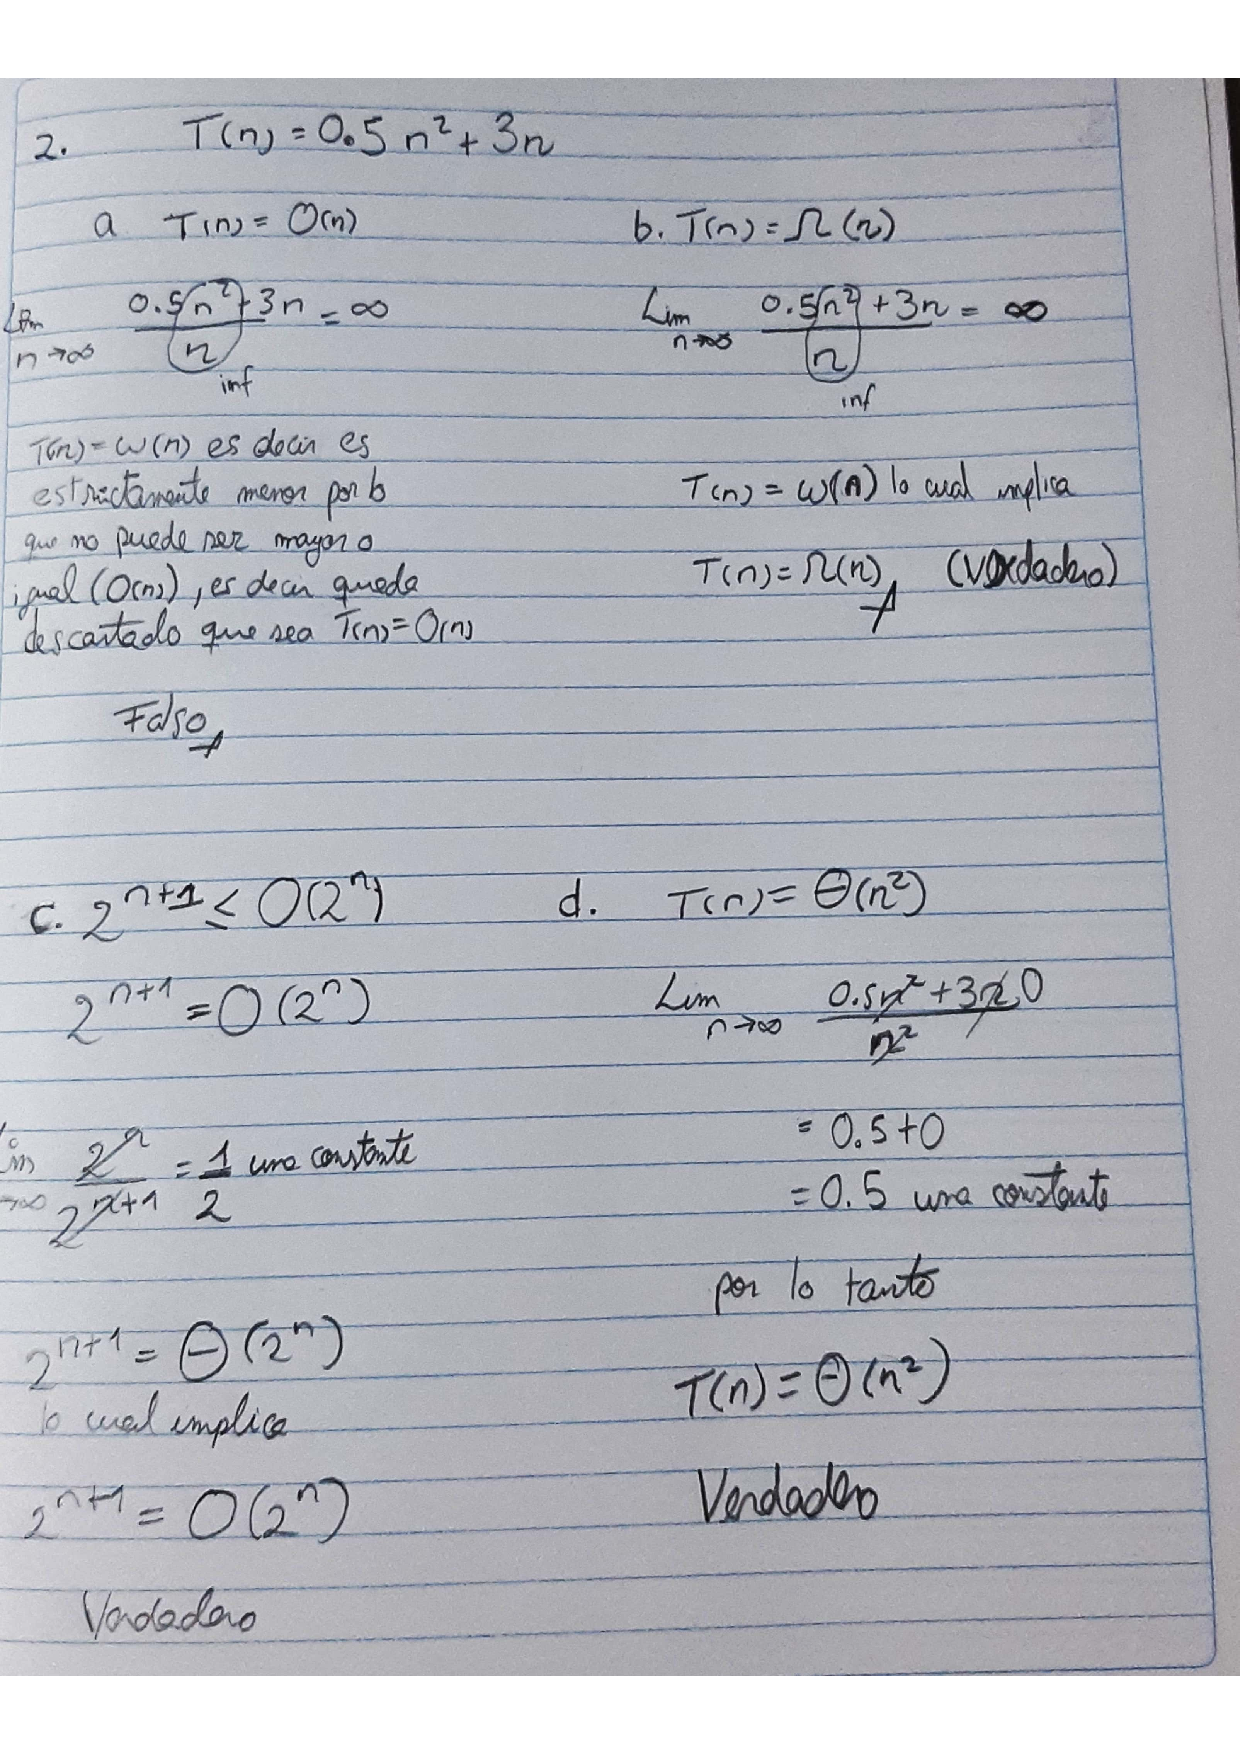
\includegraphics[width=0.9\linewidth]{problem2/problem2}%
    \end{center}
\end{problem}

\begin{problem}{Outcome b}{5}
    Consider a finite set of N points in the plane and:
    \begin{itemize}
        \item (3) Write a pseudocode of an $O(nlogn)$ divide-and-conquer algorithm to obtain the vertices of the smallest convex polygon containing all the given points.
        \item (1) Highlight the divide, conquer and combine steps on the proposed algorithm.
        \item (1) Explain the worst and best case of the algorithm and write its corresponding execution time.
    \end{itemize}

    \begin{center}
        
\includegraphics[width=0.9\linewidth]{problem3/problem3}%
    \end{center}
\end{problem}

\begin{problem}{Outcomes a, b}{3}
    Solve the following recurrences using Master Method:
    \begin{itemize}
        \item $T(n) = 4T(n/2) + n^2\sqrt{n}$
        \item $T(n) = 3T(n/2) + n$
        \item $T(n) = T(\sqrt{n}) + log(n)$
    \end{itemize}
    Hint - You can transform last expression using change of variables: $n = 2^m$
    \begin{center}
        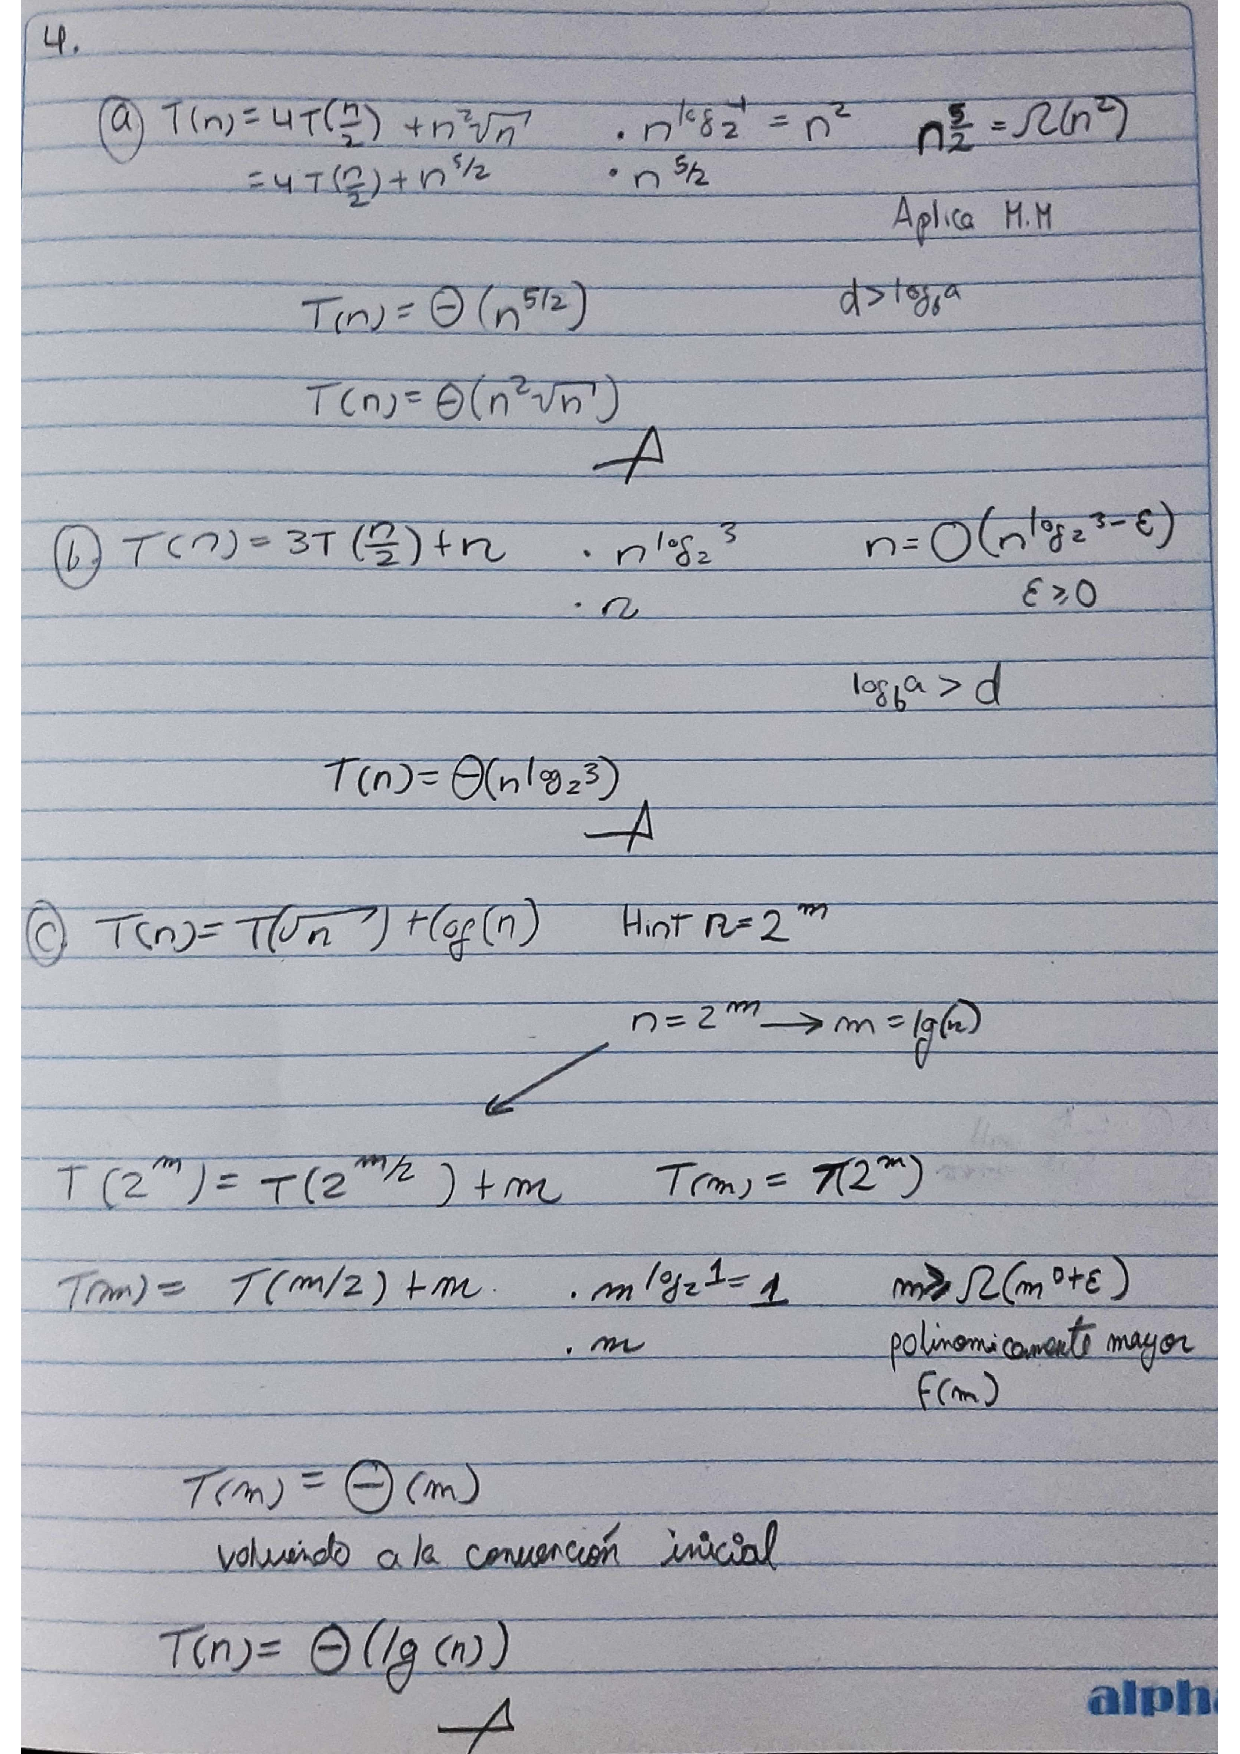
\includegraphics[width=0.9\linewidth]{problem4/problem4}%
    \end{center}
\end{problem}


\begin{problem}{Outcome a}{3}
    Prove that $T(n) = 2T(\lfloor n/2 \rfloor) + n$ is $\Theta(nlogn)$
    \begin{center}
        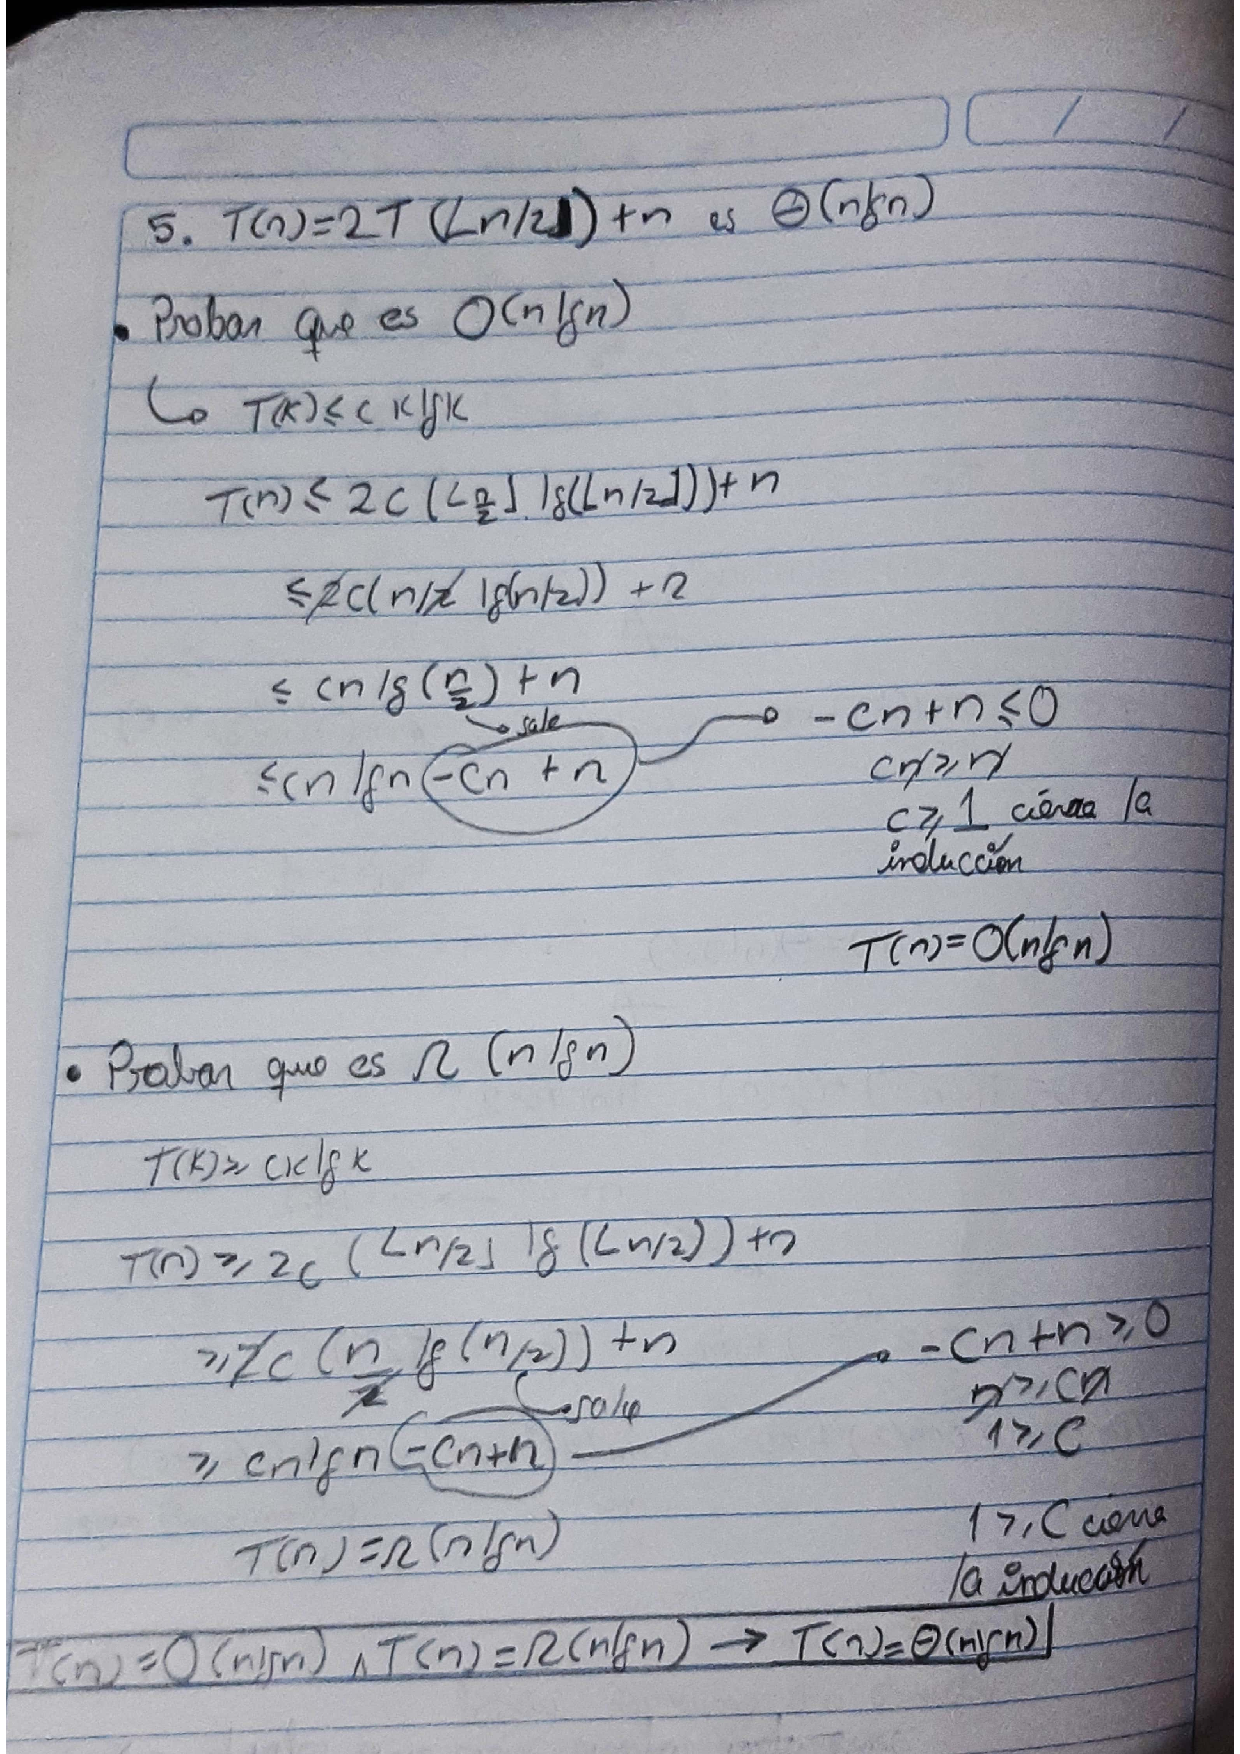
\includegraphics[width=0.9\linewidth]{problem5/problem5}%
    \end{center}
\end{problem}

\begin{problem}{Outcome b}{3}
    Given an array of N points in the Euclidean plane, write a pseudocode of a divide-and-conquer algorithm that returns the pair of points with the smallest distance between them and write the execution time of your algorithm.
    \begin{center}
        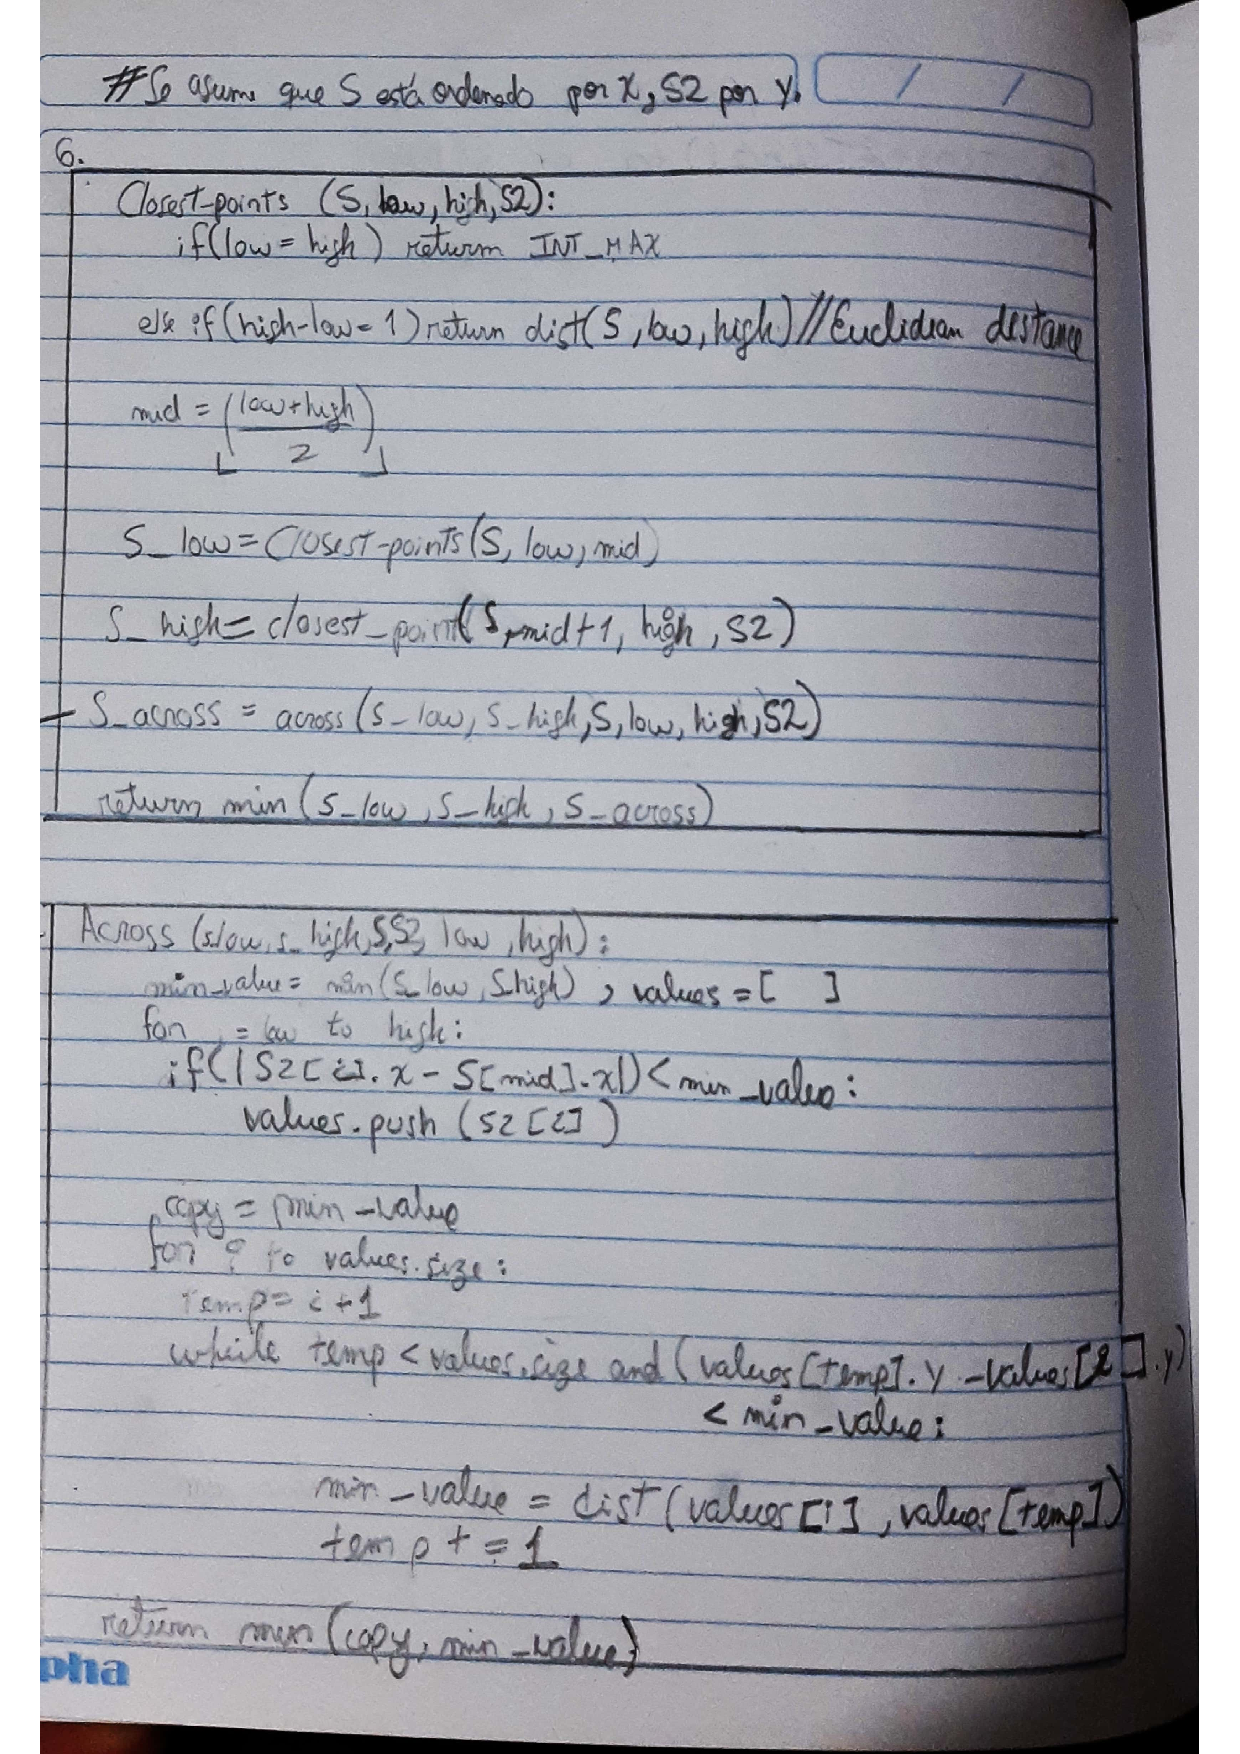
\includegraphics[width=0.9\linewidth]{problem6/problem6}%
    \end{center}
\end{problem}

\end{document}



